\chapter{\IfLanguageName{dutch}{Stand van zaken}{State of the art}}%
\label{ch:stand-van-zaken}

% Tip: Begin elk hoofdstuk met een paragraaf inleiding die beschrijft hoe dit hoofdstuk past binnen het geheel van de bachelorproef. Geef in het bijzonder aan wat de link is met
% het vorige en volgende hoofdstuk.

% Pas na deze inleidende paragraaf komt de eerste sectiehoofding.

% Dit hoofdstuk bevat je literatuurstudie. De inhoud gaat verder op de inleiding, maar zal het onderwerp van de bachelorproef *diepgaand* uitspitten. De bedoeling is dat de lezer na
% lezing van dit hoofdstuk helemaal op de hoogte is van de huidige stand van zaken (state-of-the-art) in het onderzoeksdomein. Iemand die niet vertrouwd is met het onderwerp, weet nu
% voldoende om de rest van het verhaal te kunnen volgen, zonder dat die er nog andere informatie moet over opzoeken \autocite{Pollefliet2011}.

% Je verwijst bij elke bewering die je doet, vakterm die je introduceert, enz.\ naar je bronnen. In \LaTeX{} kan dat met het commando \texttt{$\backslash${textcite\{\}}} of
% \texttt{$\backslash${autocite\{\}}}. Als argument van het commando geef je de ``sleutel'' van een ``record'' in een bibliografische databank in het Bib\LaTeX{}{}-formaat (een
% tekstbestand). Als je expliciet naar de auteur verwijst in de zin (narratieve referentie), gebruik je \texttt{$\backslash${}textcite\{\}}. Soms is de auteursnaam niet expliciet een
% onderdeel van de zin, dan gebruik je \texttt{$\backslash${}autocite\{\}} (referentie tussen haakjes). Dit gebruik je bv.~bij een citaat, of om in het bijschrift van een overgenomen
% afbeelding, broncode, tabel, enz. te verwijzen naar de bron. In de volgende paragraaf een voorbeeld van elk.

% \textcite{Knuth1998} schreef een van de standaardwerken over sorteer- en zoekalgoritmen. Experten zijn het erover eens dat cloud computing een interessante opportuniteit vormen,
% zowel voor gebruikers als voor dienstverleners op vlak van informatietechnologie~\autocite{Creeger2009}.

% Let er ook op: het \texttt{cite}-commando voor de punt, dus binnen de zin. Je verwijst meteen naar een bron in de eerste zin die erop gebaseerd is, dus niet pas op het einde van
% een paragraaf.
% ----------------------------------------------------------------------------------------------------------------------------------------------------------------------------------------------------------------------------------
Dit hoofdstuk licht toe wat een linter is en wat LaTeX (\LaTeX{}) en BibLaTeX zijn. Daarnaast wordt er meer verteld over de huidige stand van zaken binnen de wereld van BibLaTeX-linters, het toont aan waarom het gepast is om deze proof of concept uit te werken en de opportuniteiten die zich bieden binnen dit onderwerp. Alsook wordt er een diepere kijk gegeven aan andere linters hun functionaliteiten en performantie om een beter inzicht te verwerven in aspecten die van belang kunnen zijn voor het uitwerken van een eigen linter.

\section{Wat is een linter?}
Alvorens er uitgelegd wordt waarom het nuttig is om deze proof of concept uit te werken, is het belangrijk om een goed begrip te hebben van wat er effectief gemaakt wordt en wat het het nut ervan is. Het doel van deze proof of concept is om een linter te maken. Maar wat is dat juist?

\textcite{Kamunya2023} legt uit dat linten verwijst naar het proces van broncode automatisch te controleren op programmatische en stilistische fouten, dit houdt in dat een linter programmatisch je code scant om te controleren of er problemen zijn die kunnen leiden tot bugs of inconsistenties met de code-stijl en -gezondheid. De linter is hierbij de tool die ervoor gebruikt wordt.

Een linter is een statische analysetool omdat het de broncode of andere gestructureerde data analyseert zonder de code daadwerkelijk uit te voeren \autocite{Moeller2023}. Het voert een \emph{statische} analyse uit, wat betekent dat het de code inspecteert op basis van de geschreven tekst en structuur ervan, zonder rekening te houden met de daadwerkelijke uitvoering van de code.

Een linter is dus een statische analysetool, dat broncode of andere gestructureerde data kan analyseren.

\section{\LaTeX{}}
\LaTeX{} (uitspraak: LaTech), een uitbreiding op het \TeX{}-typesetting systeem van Donald E. \textcite{Knuth1984}, is bedoeld voor het opmaken van tekst en wiskundige formules. TeX werd ontwikkeld in 1977 met als doel de typografische kwaliteit te verbeteren. De stabiele versie van TeX kwam uit in 1982 en ondersteunt meerdere talen en 8-bit karakters. \LaTeX{} zelf, ontwikkeld door \textcite{Lamport1994} in 1985, voegt een reeks macro's toe om het gebruik van TeX te vereenvoudigen, en heeft zich ontwikkeld tot een standaard voor het produceren van wetenschappelijke en wiskundige documentatie \autocite{Oetiker2023}. 

\subsection{Werking}
Personen die al ervaring hebben met \LaTeX{} zullen net als \textcite{Oetiker2023} kunnen bevestigen dat \LaTeX{} functioneert door middel van commando's die de logische structuur van een document definiëren (zoals hoofdstukken, secties, en paragrafen) en dat dit anders is dan de typische WYSIWYG (What You See Is What You Get) tekstverwerkers zoals Microsoft Office Word, waar de lay-out interactief wordt bepaald tijdens het typen. \LaTeX{} vereist dat de auteur zijn tekst structureert met behulp van vooraf gedefinieerde commando's die de inleiding van het document bepalen. 

\subsection{Voordelen}
\begin{enumerate}
    \item Het biedt professionele vormgeving van lay-outs.
    \item Het ondersteunt de zetting van wiskundige formules.
    \item Het moedigt aan tot goed gestructureerd schrijven. Dit resulteert in duidelijk georganiseerde documenten.
    \item Er zijn veel uitbreidingen beschikbaar via packages om functionaliteit zoals PDF-output en betere font-ondersteuning toe te voegen.
\end{enumerate}

\subsection{Nadelen}
\begin{enumerate}
    \item Het instellen van een volledig nieuwe lay-out kan ingewikkeld en tijdrovend zijn.
    \item Niet ideaal voor zeer ongestructureerde documenten.
    \item Leercurve, de \emph{slechte} gewoontes afleren van typische WYSIWYG programma's vergt enige tijd om aan te wennen.
\end{enumerate}

\subsection{Conclusie}
\LaTeX{} \autocite{Oetiker2023} wordt vooral gewaardeerd in academische en technische kringen waar de precisie van de inhoud en de structuur voorop staan. Eens er een lay-out template bestaat, is het zeer eenvoudig om veel professionele documenten op te maken op eenzelfde manier. 
De blijvende populariteit is te dus te danken aan de uitbreidbaarheid, consistentie, brede ondersteuning van wiskundige formules, en de mogelijkheid om complexe documenten zoals proefschriften en wetenschappelijke artikelen nauwkeurig op te maken, ook wel typesetten genoemd. 
 
%--- start: BibLaTeX vs BibTeX ---
\section{BibLaTeX en BibTex} % TODO: Meer in detail gaan, technischer gaan. Uitgebreider bespreken.
BibLaTeX is een uitbreiding van \LaTeX{} die bibliografische referenties ondersteunt. Het is oorspronkelijk ontwikkeld door Philipp Lehman \autocite{Kime2024} en is een van de meest populaire bibliografische pakketten voor \LaTeX{}. BibLaTeX is een vervanging voor BibTeX, dat in 1985 werd ontwikkeld door \textcite{Patashnik1988}. BibTeX is een programma en bestandsformaat dat wordt gebruikt om bibliografische referenties te formatteren en te ordenen. BibLaTeX is een \LaTeX-pakket dat de functionaliteit van BibTeX uitbreidt en verbetert. Het biedt meer flexibiliteit en aanpassingsmogelijkheden dan BibTeX en is daarom de voorkeurskeuze voor veel \LaTeX-gebruikers.

\subsection{Compatibiliteit}
Van \textcite{Oetiker2023} kan geleerd worden dat BibLaTeX niet compatibel is met BibTeX, maar wel BibTeX-bestanden kan importeren. BibLaTeX ondersteunt UTF-8-codering, terwijl BibTeX alleen ASCII-codering ondersteunt. Gezien BibLaTeX een uitbreidig is op BibTeX, biedt het ook meer aanpassingsmogelijkheden en stijlen aan. BibLaTeX is een krachtig hulpmiddel voor het beheren van bibliografische referenties in \LaTeX-documenten en wordt veel gebruikt in academische en wetenschappelijke publicaties. 
%--- end: BibLaTeX vs BibTeX ---
\section{Huidige stand van zaken}
Op het ogenblik van het schrijven, zijn er nog geen \emph{optimale} BibLaTeX-Linters beschikbaar en de linters van de voorganger BibTex zijn niet compatibel met BibLaTeX. De enige beschikbare linter, die bestaat voor BibLaTeX voor dit moment, staat op een GitHub-repository van Pez Cuckow\footnote{\url{https://github.com/Pezmc/BibLaTeX-Linter}}. Deze hoort functioneel te zijn, maar lijkt niet optimaal wat de code betreft. Er is dus duidelijk mogelijkheid tot verbetering. De BibLaTeX-Linter van Pez Cuckow is geschreven in Python en heeft een webinterface. Naast het feit dat deze lastig werkend te krijgen was, werkt deze ook zeker niet zonder fouten. Het is mogelijk om deze effectief uit te testen, maar bij het testen werd er snel gemerkt dat er fouten optraden die niet snel op te lossen waren, zie \ref{fig:biblatex-linter-error}. Het was dus niet mogelijk om zomaar elk .bib bestand te gebruiken bij deze checker, wat het niet gunstig maakt om te gebruiken. Wel was het interessant om te kijken hoe Cuckow bepaalde aspecten interpreteerde en uitvoerde. Dit was uiteindelijk ook een bron waaruit inspiratie gehaald kon worden.

\begin{figure}[ht]
    \centering
    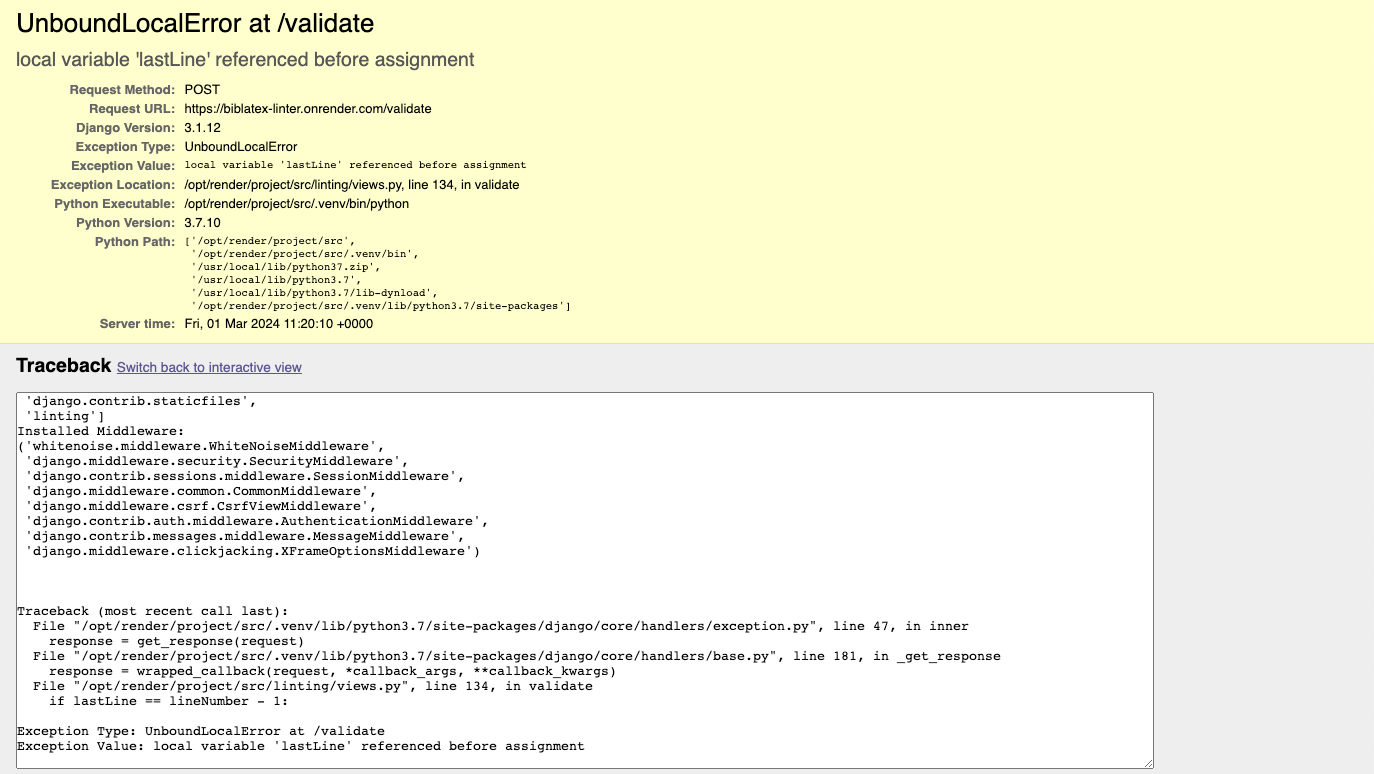
\includegraphics[width=0.7\textwidth]{./files/Pezmc-LinterError_cropped.png}
    \caption[Foutmelding BibLaTeX-linter]{Lintingerror bij het valideren van een BibLaTeX bestand, gebruikmakende van de linter geschreven door Pez Cuckow.}
    \label{fig:biblatex-linter-error}
\end{figure}

Daarnaast leek de aanpak van de geschreven code ook niet optimaal te zijn op vlak van leesbaarheid en uitbreidbaarheid. Gezien dit echter wel criteria zijn waar de proof of concept aan moest voldoen, werd er besloten om deze linter niet verder te onderzoeken. Er werd wel gekeken naar de functionaliteiten die deze linter aanbood en andere zaken die handig leken om over te nemen in de eigen implementatie.

\section{Andere linters}
Gezien het wat BibLaTeX linters betreft zeer beperkt is, werd er op zoek gegaan naar andere soorten linters. Bijvoorbeeld een linter voor JavaScript, Python of andere programmeertalen. Er werd gekeken naar het soort features dat de linters aanbieden, hun performantie, alsook als hun broncode indien deze toegankelijk was. Enkele linters die bekeken werden zijn: JSHint, Stylelint, Ruff, PyType en bibl. Net als de proof of concept, waren al de bekeken linters gratis te gebruiken en open source.

Daaruit bleek dat naast de manier van implementeren, de taal waaruit de linter opgebouwd is ook van belang is voor de performantie. Dit was het begin naar een onderzoek voor de ideale programmeertaal te vinden voor deze proof of concept. 

\subsection{Ruff}
% Ruff is een Python linter die door \textcite{Astral2024} ontwikkeld is. In vergelijking met andere Python linters is Ruff veel performanter. Dit is omdat Ruff in tegenstelling tot de concurrenten, geschreven is in Rust in plaats van Python. Op de website van Astral, makers van Ruff, is er een vergelijking te zien tussen Ruff en andere Python linters die wel in Python geschreven zijn. Astral is niet de enige die dit aantoont, ook \textcite{TurnerTrauring2023} schrijft in een artikel dat de snelheid van Ruff zeker merkbaar is en toont dit aan met behulp van uitgevoerde tests. Vooral bij pipelines op virtuele machines gezien deze vCPU's (virtuele processor units) gebruiken en deze meestal trager zijn dan de processing units die terug te vinden zijn in moderne laptops of desktops.
Ruff\footnote{\url{https://astral.sh/ruff}} is een Python linter ontwikkeld door \textcite{Astral2024}, geschreven in de programmeertaal Rust. Dit onderscheidt Ruff van andere Python linters, die doorgaans in Python zelf zijn geschreven. Rust staat bekend om zijn snelheid en veiligheid, wat het een uitstekende keuze maakt voor een linter. Bovendien is Rust lichter om op hardware te draaien dan Python, aangezien Python een interpretatieve taal is en Rust een gecompileerde taal. Dit maakt Ruff bijzonder geschikt voor gebruik in CI-pipelines. 

Een ander belangrijk voordeel van Rust is de stabiliteit van de taal. Er is slechts één versie van Rust en die wordt continu doorontwikkeld, wat ervoor zorgt dat code die vandaag gecompileerd wordt, ook over tien jaar nog gecompileerd kan worden. Dit biedt een aanzienlijke zekerheid voor de toekomstbestendigheid van software.

Ruff kan op bepaalde taken tien tot wel honderd keer sneller zijn dan zijn concurrenten. Dit wekt vanzelfsprekend de interesse om de prestaties van de Rust-taal te testen. Op de website van Astral, de makers van Ruff, is een vergelijking te vinden tussen Ruff en andere Python linters. Ook \textcite{TurnerTrauring2023} bevestigen in hun artikel dat de snelheid van Ruff duidelijk merkbaar is en onderbouwen dit met testresultaten. Deze prestaties zijn vooral voordelig in pipelines op virtuele machines, aangezien vCPU's (virtuele processor units) meestal trager zijn dan de verwerkingsunits in moderne laptops of desktops.

\subsection{DirtyRat}
\label{subsec:dirtyrat}
DirtyRat is een JavaScript linter waar op gebotst werd tijdens het onderzoeken naar hoe een linter gemaakt kon worden. Het is een linter die zelf in JavaScript geschreven is en waarvan de stapsgewijze opbouw te vinden is in het artikel van \textcite{BorgesLate2021}. Daarnaast is ook de broncode zelf te vinden op GitHub\footnote{\url{https://github.com/JoanaBLate/dirtyrat}}. Dit was ook de reden waarom er besloten werd om JavaScript als kandidaat-programmeertaal te nemen. 

Hoewel het artikel zeer in detail gaat en het grondig onderzocht werd, werd er vastgesteld dat het toch wat te uitgebreid is voor deze proof of concept. JavaScript en andere programmeertalen zitten met veel meer complexe structureren dan een BibLaTeX bestand. Dus hoewel het interessant was om te zien hoe een linter in JavaScript gemaakt kon worden, was het dus zeker niet nodig om elke component over te nemen.


\subsection{Bibl}
Bibl\footnote{\url{https://gitlab.com/arnevdk/bibl}} is een linter voor BibTeX, de voorloper van BibLaTeX, geschreven in Python door Arne Van Den Kerchove. Het onderzoeken van een linter voor de voorloper van BibLaTeX leek bijzonder interessant om een goed inzicht te krijgen in wat precies verwacht kan worden van een linter. Bibl biedt een uitgebreide lijst van regels, evenals een gedetailleerde projectstructuur en implementatiewijze van zowel de lintercode als de bijbehorende tests.

Bibl werd ontdekt net voordat er begonnen werd met de ontwikkeling van een eigen linter. Na een grondige analyse bleek dat Bibl een goed opgebouwde, modulaire en efficiënte open-source linter is. Bibl voldeed aan vrijwel alle criteria die voor de proof of concept linter waren opgesteld, wat leidde tot een nieuwe visie.

Het maken van een linter zoals Bibl, maar dan voor BibLaTeX in plaats van BibTeX, leek een haalbaar einddoel. Echter, vanwege een achterstand op de planning, zou het niet mogelijk zijn om een eigen linter even uitgebreid uit te werken. Hoewel het concept van een proof of concept wellicht bereikt kon worden, leek het voordeliger om Bibl te proberen gebruiken en compatibel te maken met BibLaTeX.

Gezien de verschillen tussen BibTeX en BibLaTeX, was er enige twijfel over de haalbaarheid hiervan, vooral omdat Bibl gebruik maakt van pybtex als parser. Op de site van pybtex\footnote{\url{https://pybtex.org/}} staat het volgende vermeld:

\begin{quote}\emph{Pybtex is a BibTeX-compatible bibliography processor written in Python.}\end{quote}

Dit impliceert dat pybtex verantwoordelijk is voor het extraheren van gegevens uit bibliografiebestanden. Hoewel de quote niet expliciet vermeldt dat het alleen voor BibTeX-bestanden werkt, wordt compatibiliteit met BibLaTeX nergens expliciet genoemd. Het was dus noodzakelijk om dit zelf te testen.

Voor de test werd een BibLaTeX-document gebruikt dat door de promotor was gedeeld. Dit document bevatte geldige bronvermeldingen en was daarmee perfect geschikt om te onderzoeken of Bibl als basis gebruikt kon worden. Bibl werd snel geïnstalleerd via de Python package manager, pip. Vervolgens werd het lint-commando uitgevoerd op het BibLaTeX-document en werd bekeken wat Bibl rapporteerde.

Bibl crashte niet en genereerde een uitgebreide lijst opmerkingen; dit was een positief resultaat. Er waren echter enkele bestaande regels die niet compatibel waren met BibLaTeX-bestanden. 

\subsubsection{Algemene structuur}
\begin{figure}[ht]
    \centering
    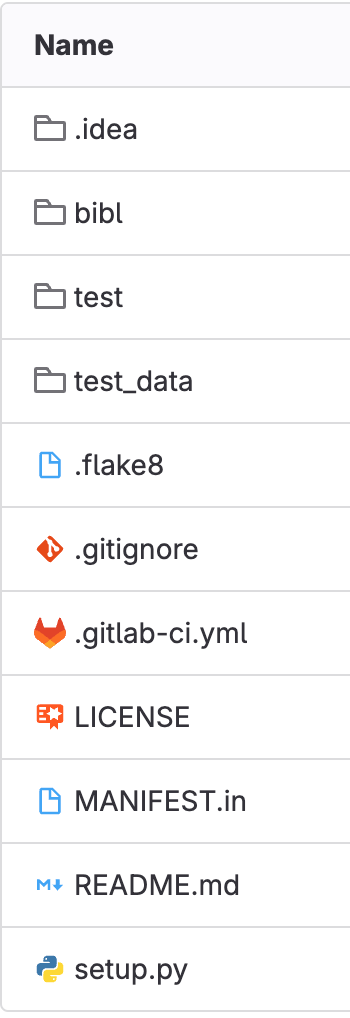
\includegraphics[width=0.3\textwidth]{./files/bibl_repo.png}
    \caption[bibl repository]{Repository overzicht bibl.}
    \label{fig:bibl_repo}
\end{figure}

De gitlab-repository van bibl\footnote{\url{https://gitlab.com/arnevdk/bibl}} is een goed voorbeeld van hoe een goed gestructureerd project eruit kan zien. Naast de bibl folder, die alle broncode van bibl zelf bevat, zijn er ook: testen, test-data, lintervoorkeuren, een pipeline, een licentie, een duidelijke readme en een installatie-script aanwezig. Ook de .idea, .gitignore en MANIFEST.in zijn niet onbelangrijk. de .idea bevat de voorkeursinstellingen voor de IDE (Integrated development environment, ook gekend als werkomgeving) van de auteur, het .gitignore bestand bevat een opsomming van bestanden of soort bestanden die niet op de repository dienen te komen. Denk hier aan tijdelijke bestanden die vanzelf aangemaakt worden; deze zijn niet nodig op de repository omdat ze onnodig plaats gebruiken. Tot slot wordt het MANIFEST.in bestand in Python wordt gebruikt om aan te geven welke bestanden moeten worden opgenomen bij het maken van een distributiepakket; wat nodig is om het beschikbaar te stellen bij de pakketbeheerder\footnote{\url{https://pypi.org/}} (pip).

\section{bibl pakket - diepere blik}
\begin{figure}[ht]
    \centering
    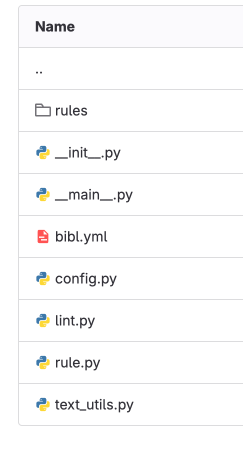
\includegraphics[width=0.4\textwidth]{./files/bibl_src.png}
    \caption[bibl repository]{Repository overzicht bibl broncode.}
    \label{fig:bibl_src}
\end{figure}

De structuur van bibl \ref{fig:bibl_src} volgt een gebruikelijke pakket-gebaseerde aanpak voor het organiseren van code. Deze aanpak wordt vaak toegepast wanneer een project is opgezet als een herbruikbaar pakket, in plaats van een los script. De aanwezigheid van `\_\_init\_\_.py` zorgt er namelijk voor dat het pakket importeerbaar is \autocite{Loubser2021}. Dit is direct ook een indicator dat het om een pakket gaat.

Om bibl te begrijpen, wordt de broncode van bibl zelf geanalyseerd.

\subsection{\_\_init\_\_.py}
Zoals eerder vermeld, is dit bestand kenmerkend bij pakketten. Het bestand is namelijk vereist voor Python om de directory als een pakket te behandelen. Het kan leeg zijn, maar het kan ook initialisatiecode of pakket-niveau-definities bevatten; in dit geval bevat het de huidige softwareversie.

\subsection{\_\_main\_\_.py}
Dit bestand wordt gebruikt wanneer het pakket als een script wordt uitgevoerd (bijvoorbeeld python -m bibl). Het bevat de implementatie van de Command Line Interface (CLI) voor het linten van bibliografische bestanden in BibTeX-formaat. Het script, hiervoor als referentie bestand, maakt gebruik van de \texttt{Click}-bibliotheek om een gebruiksvriendelijke interface te bieden voor het controleren van bibliografische referenties op consistentie en correctheid. Hieronder volgt een overzicht van de verschillende onderdelen binnen dit bestand.

\subsubsection{Imports en Configuratie}

Het script begint met het importeren van noodzakelijke modules en functies, waaronder \texttt{Click} voor het CLI-framework, en functies uit de \texttt{bibl}-module voor linting, configuratie en regels:

\begin{minted}[autogobble, breaklines, linenos, samepage]{python3}
import os
import warnings
import click
from bibl import __version__
from bibl.lint import lint as bibl_lint
from bibl.config import load_config_file, set_config
from bibl.rule import load_rules
from bibl.text_utils import format_rules_markdown_tables
\end{minted}

\subsubsection{CLI Basisgroep}

Een CLI basisgroep functioneert als een container, of groepering, voor meerdere gerelateerde command-line commando's. Hiermee wordt het mogelijk gemaakt om een hoofdcommando te definiëren waaraan subcommando's kunnen worden toegevoegd.
De basisgroep wordt gedefinieerd met behulp van de \texttt{@click.group()} decorator. Deze groep fungeert als een container voor subcommando's die specifieke taken uitvoeren. De subcommando's kunnen tegelijkertijd ook als parameter beschouwd worden. Opties die van toepassing zijn op de gehele groep kunnen hier ook worden gespecificeerd. Een voorbeeld van de definitie van een basisgroep in het script is als volgt:

\begin{minted}[autogobble, breaklines, linenos]{python3}
@click.group()
@click.option('-c', '--config', help='Custom configuration file path.', type=str)
@click.option('--select', help='Comma separated list of enabled rules, all other rules will be disabled.', type=str)
@click.option('--ignore', help='Comma separated list of disabled rules, all other rules will be enabled.', type=str)
@click.option('--indent-spaces', help='Number of trailing whitespaces for indented line, used by TO1.', type=int)
@click.option('--max-line-length', help='Max line length before wrap recommended, used by T03.', type=int)
def cli(config, select, ignore, indent_spaces, max_line_length):
    if config is not None:
        load_config_file(config)
    elif os.path.isfile('bibl.yml'):
        load_config_file('bibl.yml')
    elif os.path.isfile('.bibl.yml'):
        load_config_file('.bibl.yml')
    if select is not None:
        set_config('select', select.split(','))
    if ignore is not None:
        set_config('ignore', ignore.split(','))
    set_config('indent_spaces', indent_spaces)
    set_config('max_line_length', max_line_length)
\end{minted}

\subsubsection{Lint Commando}

Het \texttt{lint} commando lint één of meer opgegeven BibTeX-bestanden:

\begin{minted}[autogobble, breaklines, linenos, samepage]{python3}
@cli.command(help="Lint a BibTeX bibliography file.")
@click.argument('bibliography', type=str, nargs=-1)
def lint(bibliography):
    warnings.filterwarnings("ignore")
    for bib in bibliography:
        bibl_lint(bib)
\end{minted}

\subsubsection{Lijst Commando's}

Er zijn twee commando's om de lintingregels weer te geven: \texttt{list\_all} toont alle beschikbare regels, terwijl \texttt{list\_enabled} alleen de ingeschakelde regels toont.

\begin{minted}[autogobble, breaklines, linenos]{python3}
@cli.command(help="Show all available rules.")
@click.option('-m', 'markdown', help='Format rules as markdown table.', is_flag=True)
def list_all(markdown):
    rules = load_rules().all
    if markdown:
        click.echo(format_rules_markdown_tables(rules))
    else:
        for rule in rules:
            click.echo(rule)

@cli.command(help="Show all rules enabled by the configuration.")
@click.option('-m', 'markdown', help='Format rules as markdown table.', is_flag=True)
def list_enabled(markdown):
    rules = load_rules().enabled
    if markdown:
        click.echo(format_rules_markdown_tables(rules))
    else:
        for rule in rules:
            click.echo(rule)
\end{minted}

\subsubsection{Versie Commando}

Het \texttt{version} commando toont de huidige versie van het \texttt{bibl}-pakket:

\begin{minted}[autogobble, breaklines, linenos, samepage]{python3}
@cli.command(help="Show the package version.")
def version():
    click.echo('bibl version: ' + __version__)
\end{minted}

\subsubsection{Hoofdprogramma}

Het hoofdprogramma start de CLI met \texttt{cli(prog\_name='bibl')}:

\begin{minted}[autogobble, breaklines, linenos, samepage]{python3}
if __name__ == '__main__':
    cli(prog_name='bibl')
\end{minted}
%---
\subsection{bibl.yml}
Het volgende configuratiebestand is een YAML (.yml) bestand dat de standaardinstellingen voor de bibliografische lintingtool definieert. Dit bestand specificeert welke regels ingeschakeld of uitgeschakeld moeten worden, evenals andere configuratie-opties zoals de maximale regellengte en het aantal inspringende spaties.

\begin{minted}[autogobble, breaklines, linenos]{yaml}
## DEFAULT BIBL CONFIG
select: [ ] # List of enabled rules, all other rules will be disabled
ignore: [ ] # List of disabled rules, all other rules will be enabled
# Specify max 1 of the two options above. If none are specified, all rules will be enabled
indent_spaces: 4 # number of trailing whitespaces for indented line, used by TO1
max_line_length: 120  # max line length before wrap recommended, used by T03
abbreviation_dot: True  # abbreviate middle names with dot (John F. Kennedy) as opposed to without (John F Kennedy), used by E02

# Specification from https://en.wikipedia.org/wiki/BibTeX extended with fields used in JabRef.
# This specification is used to generate M01 and U01 rules
type_spec:
  article: # An article from a journal or magazine.
    required: [ title, journal, year, volume ]
    optional: [ number, pages, month, doi, key, file ]
  book: # A book with an explicit publisher.
    required: [ title, publisher, year ]
    optional: [ volume, number, series, address, edition, month, key, url, file, isbn ]
# NOTE: Overige entry types weggelaten wegens plaats!
\end{minted}

\subsubsection{Beschrijving van de Configuratieopties}

De YAML-configuratie begint met het definiëren van een aantal algemene opties voor de linter:

\begin{itemize}
    \item \texttt{select}: Een lijst van ingeschakelde regels. Indien gespecificeerd, worden alle andere regels uitgeschakeld.
    \item \texttt{ignore}: Een lijst van uitgeschakelde regels. Indien gespecificeerd, worden alle andere regels ingeschakeld.
    \item \texttt{indent\_spaces}: Het aantal inspringende spaties voor ingesprongen regels, gebruikt door de regel TO1.
    \item \texttt{max\_line\_length}: De maximale regellengte voordat een regel wordt afgebroken, aanbevolen door de regel T03.
    \item \texttt{abbreviation\_dot}: Bepaalt of middelste namen met een punt worden afgekort (bijvoorbeeld John F. Kennedy) of zonder punt (bijvoorbeeld John F Kennedy), gebruikt door de regel E02.
\end{itemize}

\subsubsection{Type Specificaties}

Daarnaast bevat het configuratiebestand een specificatie van verschillende typen BibTeX-entries en hun vereiste en optionele velden. Deze specificatie is gebaseerd op de standaard BibTeX-specificatie en is uitgebreid met velden die worden gebruikt in JabRef. Deze specificatie wordt gebruikt om de regels M01 en U01 te genereren.
Hieronder zijn er enkelen opgelijst, maar let op, het zijn ze niet allemaal! Raadpleeg de gehele lijst op de GitLab-repository van bibl\footnote{\url{https://gitlab.com/arnevdk/bibl/-/blob/master/bibl/bibl.yml}}
\begin{itemize}
    \item \texttt{article}: Een artikel uit een tijdschrift of magazine. Vereist velden zoals \texttt{title}, \texttt{journal}, \texttt{year}, en \texttt{volume}.
    \item \texttt{book}: Een boek met een expliciete uitgever. Vereist velden zoals \texttt{title}, \texttt{publisher}, en \texttt{year}.
    \item \texttt{booklet}: Een werk dat is gedrukt en gebonden, maar zonder een genoemde uitgever of sponsorende instelling. Vereist het \texttt{title} veld.
    \item ...
\end{itemize}

Deze configuratie-instellingen en type-specificaties vormen de basis voor het configureren en uitvoeren van de bibliografische lintingtool, waarbij consistentie en correctheid van de bibliografische gegevens worden gewaarborgd.

% --------------
\subsection{config.py}
% TODO : Continue here! :)

\subsection{lint.py}

\subsection{rule.py}

\subsection{text\_utils.py}
% \begin{itemize}

%     \item \textbf{config.py}: Hier wordt het standaard configuratie bestand ingesteld op bibl.yml en wordt er ook de logica bijgehouden om te weten hoe het configuratiebestand geïnterpreteerd dient te worden.
%     \item \textbf{lint.py}: Dit bestand bevat de algemene linter logica.
% \end{itemize}





rule.py: Dit bestand bevat waarschijnlijk de implementatie van regels of algoritmes specifiek voor het "bibl"-project. Het kan klassen, functies of methoden definiëren gerelateerd aan de kernfunctionaliteit van de toepassing.
text\_utils.py: Dit bestand bevat waarschijnlijk hulpprogramma's of klassen gerelateerd aan tekstverwerking, -manipulatie of -analyse. Het kan algemene bewerkingen bieden die worden gebruikt in verschillende delen van het project.

De structuur volgt de standaard Python-pakketlay-out, wat het gemakkelijk maakt om het project te distribueren, te installeren en te gebruiken. Door de bestanden te organiseren in een pakket, kan men modules importeren en functionaliteit van andere delen van het project gebruiken met behulp van relatieve imports (bijvoorbeeld from . import rule).


% ----
\section{Programmeertaal}
Wat de programmeertaal voor de proof of concept betreft, werd er zich beperkt tot Rust, Python en JavaScript. Er werd een beperkt prototype uitgewerkt in elk van deze talen en deze werden met elkaar vergeleken om te bepalen welke taal het meest geschikt was. Alle opties zijn cross-platform, wat belangrijk is gezien de linter bruikbaar dient te zijn voor iedereen. Alsook dient het een programmeertaal te zijn die gekend is, hiermee wordt er bedoeld dat het een programmeertaal moet zijn die al matuur is en door een groot aantal mensen gekend is.

\subsection{Rust}
Gezien de performantie van Ruff, leek Rust een gepaste optie om de linter in te maken. Ook de stijgende populariteit van de taal maakt dit een aantrekkelijke optie. Ondanks dat dit een onbekende taal is, leek het zeker wel een interessante taal om te leren. De haalbaarheid van de proof of concept kwam echter meer in gevaar door deze keuze. Hoewel de populariteit stijgt, blijft het wel nog een taal die niet door iedereen gekend is, in tegenstelling tot bijvoorbeeld JavaScript of Python. Een ander groot pluspunt aan Rust is dat code die vandaag compiled, ook nog binnen vijf of tien jaar zal kunnen compilen. Dit omdat de makers ervoor streven dat het een super compatibele programmeertaal is. Wat men niet met volle zekerheid van bijvoorbeeld Python\footnote{\url{https://devguide.python.org/versions/}} zou kunnen zeggen. 
 
Dankzij \textcite{Klabnik2022} kan er geleerd worden dat Rust een nadruk legt op typeveiligheid (typesafety) en geheugenveiligheid. Wanneer een taal of systeem geheugenveilig is, betekent dit dat het ontworpen is om toegangsfouten zoals bufferoverlopen, dangling pointers (verwijzingen naar vrijgegeven geheugen), en dubbele bevrijdingen van geheugen (double frees) te voorkomen. Deze soorten fouten kunnen leiden tot onvoorspelbaar gedrag, crashes, en beveiligingslekken zoals het uitvoeren van willekeurige code of informatie-lekken. Het is dus een goede eigenschap om te hebben.

\subsection{Python}
Python was wellicht stukken trager in vergelijking met Rust in de test die gevonden werd, maar het blijft wel een taal waar iedereen gemakkelijk mee kan beginnen te werken. Voor het gemak van uitbreidbaarheid is dit dan weer een interessante optie om deze taal in optie te nemen. Zoals eerder vermeld door \textcite{TurnerTrauring2023} zou de performantie vooral bij de pipeline te merken zijn.
De echte vraag blijft momenteel nog altijd in hoeverre het minder performant zijn een grote zorg zal worden voor deze proof of concept.

\subsection{JavaScript}
Een zeer gekende scripting taal dat cross-platform gebruikt kan worden. Hoewel het eerder gericht is voor het gebruik in websites of GUI gerichte scripts, is het ook mogelijk om er cli-tools mee te maken. De performantie werd onderzocht. JavaScript is ook een dynamisch typerende taal, wat in theorie voor problemen zou kunnen zorgen in sommige use-cases, al leek dit geen zorg te zijn voor deze proof of concept\autocite{Simpson2023}.

% ----
\section{Opbouw linter}
Aan het begin van dit project werd de beslissing genomen om direct met de ontwikkeling van een prototype aan de slag te gaan, wat leidde tot de zoektocht naar geschikte bronnen. Deze beslissing werd genomen gezien de beperkte tijd en de hoeveelheid aan onderzoek die diende te gebeuren. Indien Rust de taal zou moeten worden, moest deze nog volledig aangeleerd worden en zou er immers geen kostbare tijd verloren mogen gaan.
In dit proces werden de artikelen van \textcite{BorgesLate2021}, die een stapsgewijze handleiding bieden voor het bouwen van een JavaScript-linter, als bijzonder nuttig beschouwd. Ondanks dat de lectuur van deze serie aanvankelijk de indruk wekte dat het project complexer zou zijn dan verwacht, veranderde dit vermoeden na verder onderzoek naar de structuur van .bib-bestanden. Het werd duidelijk dat de ontwikkeling van een linter voor BibLaTeX minder complex is dan voor programmeertalen. Dit is te wijten aan het feit dat programmeertalen loops, conditionele statements en een scala aan andere complexe elementen bevatten, terwijl BibLaTeX gekenmerkt wordt door een consistente en gestandaardiseerde structuur, waardoor de noodzaak voor het opleggen van regels aanzienlijk vermindert. Het was echter wel zeer nuttig om alle componenten te zien die aan bod kunnen komen bij het bouwen van een linter en om deze in gedachte te houden voor de effectieve uitwerking van de BibLaTeX-linter proof of concept.

\section{Open-source}
Deze proof of concept heeft als visie om open source te zijn zodat iedereen er gebruik van kan maken en ook iedereen in staat is om een bijdrage te leveren.
Open-source software voldoet aan specifieke criteria die het een waardevolle en veelzijdige keuze maken. Onder deze criteria verstaat men iets als open-source zijnde:
\begin{itemize}
    \item \textbf{Vrij verspreid} kan worden, waardoor het voor iedereen toegankelijk is.
    \item De \textbf{broncode beschikbaar stelt}, zodat ontwikkelaars het kunnen begrijpen, aanpassen en verbeteren.
    \item \textbf{Modificaties en afgeleide werken} toestaat, waardoor een levendige gemeenschap van bijdragers ontstaat.
    \item De \textbf{integriteit van de oorspronkelijke broncode waarborgt}, zodat de software betrouwbaar blijft.
    \item \textbf{Niet discrimineert} op basis van personen of groepen, en voor iedereen toegankelijk is.
    \item \textbf{Niet beperkt is tot specifieke vakgebieden}, waardoor het breed inzetbaar is.
    \item \textbf{Rechten toepast op alle partijen} die de software verspreiden, wat eerlijkheid bevordert.
    \item \textbf{Niet afhankelijk is van een specifieke software distributie}, waardoor het flexibel blijft.
    \item \textbf{Geen beperkingen oplegt aan andere software} die ermee wordt verspreid, wat samenwerking stimuleert.
    \item \textbf{Technologie-neutraal} is, zodat het zich kan aanpassen aan veranderende omstandigheden.
\end{itemize}

Kortom, open-source is toegankelijk, krachtig en bevordert innovatie in de digitale wereld voor iedereen \autocite{OpenSource2006}.

\section{Kanban}
Overzichtelijk te werk gaan is voor elk project van belang. Ook bij het ontwikkelen van deze proof of concept was er geen uitzondering. Om een simplistisch maar effectief overzicht te behouden, werd er een kanbanbord gebruikt.

Een Kanban-bord is een visueel hulpmiddel dat teams gebruikt voor het beheren van projecttaken.

De belangrijkste onderdelen van een Kanban-bord zijn de kaarten en kolommen. Kaarten vertegenwoordigen individuele taken en bevatten details zoals beschrijvingen en deadlines. Kolommen vertegenwoordigen verschillende stadia van de workflow, zoals 'te doen', 'bezig', en 'gedaan'. Het beperken van het aantal taken in uitvoering zorgt voor efficiënter werken door de focus te behouden en afleiding te verminderen.

Kanban-borden maken gebruik van zes kernpraktijken: de workflow visualiseren, het werk in uitvoering beperken, workflows beheren, expliciete beleidsregels implementeren, ruimte voor feedback bieden, en voortdurend zoeken naar verbetering. Elk van deze praktijken draagt bij aan het verhogen van flexibiliteit, het reduceren van downtime en het verhogen van de efficiëntie binnen teams \autocite{Hennigan2024}.

Zoals eerder vermeld, werd er binnen deze proef ook een simpele vorm van een kanbanbord gebruikt om een overzicht te bewaren van welke functionaliteiten er al dan niet afgewerkt waren. Dit was handig om te weten of de MVP (Minimum Viable Product) gehaald kon worden tegen de deadline.
